\begin{frame}{Programa de PC para la transmisión de datos}
	\framesubtitle{hacia y desde el FPGA}
	\begin{columns}
		\begin{column}{.4\textwidth}
			\centering
			\begin{tikzpicture}[scale=.8,>=latex]
				\begin{scope}[transform shape,node distance=1]
					\node[mealy]	(init)	[]{Inicializacion;};
					\node[mealy] (snd) [below=of init]{Generar Datos;\\Enviar Datos;}
						edge[<-] (init);
					\node[mealy] (rcv) [below=of snd]{Recibir Datos;}
						edge[<-] (snd);
					\draw[<-] (rcv) to [in=0,loop,looseness=5] (rcv);
					\node[mealy](cmpr)[below=of rcv]{Comparar;\\Guardar en\\\hspace{2ex}archivo;}
						edge[<-] (rcv);
					\draw[->] (cmpr) to [in=180,out=180,loop,looseness=1] (snd);
				\end{scope}
				\begin{scope}
					\only<2>{\node[ellipse,ultra thick,draw=blue,fit=(init)]{};}
					\only<3>{\node[ellipse,ultra thick,draw=blue,fit=(snd)]{};}
					\only<4>{\node[ellipse,ultra thick,draw=blue,fit=(rcv)]{};}
					\only<5>{\node[ellipse,ultra thick,draw=blue,fit=(cmpr)]{};}
				\end{scope}
			\end{tikzpicture}
		\end{column}
		\begin{column}{.6\textwidth}
			\only<1>{Se realizó un programa de computadoras, escrito en lenguaje C, para el cual se utilizó la biblioteca \texttt{libusb-1.0}, que permite obtener acceso al puerto USB como así también transmitir y recibir datos a través de él.}
			\only<2>{Inicialización:
				\begin{itemize}
					\item Se listan los dispositivos
					\item Se busca y selecciona el adecuado
					\item Se configura la interfaz
				\end{itemize}
			}
			\only<3>{Generar Datos:\\
				\centering
				\begin{tikzpicture}[scale=.5]
					\begin{scope}[transform shape,node distance=.2,>=latex,]
						\draw[step=1] (.1,.1) grid (3.9,3.9);
						\node (a11) at (0.5,3.5){0};
						\node (a12) at (1.5,3.5){0};
						\node (a13) at (2.5,3.5){1};
						\node[color=red] (a18) at (3.5,3.5){1};
						\node [left=of a11,anchor=east] {\small{Fila 1}};
						\node[above=of a18,align=center]{Paridad\\columna};
						
						\node (a21) at (0.5,2.5){1};
						\node (a22) at (1.5,2.5){1};
						\node (a23) at (2.5,2.5){0};
						\node[color=red] (a28) at (3.5,2.5){0};
						\node [left=of a21,anchor=east] {\small{Fila 2}};
						
						\node (a31) at (0.5,1.5){0};
						\node (a32) at (1.5,1.5){1};
						\node (a33) at (2.5,1.5){0};
						\node[color=red] (a38) at (3.5,1.5){1};
						\node [left=of a31,anchor=east] {\small{Fila 3}};
						
						\node[color=red] (a81) at (0.5,0.5){1};
						\node[color=red] (a82) at (1.5,0.5){0};
						\node[color=red] (a83) at (2.5,0.5){1};
						\node[color=red] (a84) at (3.5,0.5){0};
						\node [left=of a81,anchor=east] {Paridad fila};
					\end{scope}
					\begin{scope}[on background layer]
						\node[rounded corners,rectangle,fit={(a18)(a84)},fill=gray!20] {};
						\node[rounded corners,rectangle,fit={(a81)(a84)},fill=gray!20] {};
					\end{scope}
				\end{tikzpicture}\\
				\begin{itemize}
					\item Se generan datos aleatorios de 7 bits
					\item Se agrega un bit de paridad.
					\item Cada 7 bytes generados, se agrega 1 Byte con las paridades verticales.
					\item Se generan 16 tramas de 8 bytes, para alcanzar un paquete de 128 Bytes de datos. 
				\end{itemize}				
			}
		\only<4>{Recibir datos:\\Se solicita la recepción de datos y se espera hasta que estos lleguen}
		\only<5>{Comparar:\\
			\begin{itemize}
				\item Se chequea que los datos recibidos no tuvieron errores.
				\item Se comparan los datos recibidos con los enviados.
			\end{itemize}
			Guardar en archivo;\\
		}
		\end{column}
	\end{columns}
\end{frame}

\begin{frame}{Sistema en funcionamiento}
	\centering
	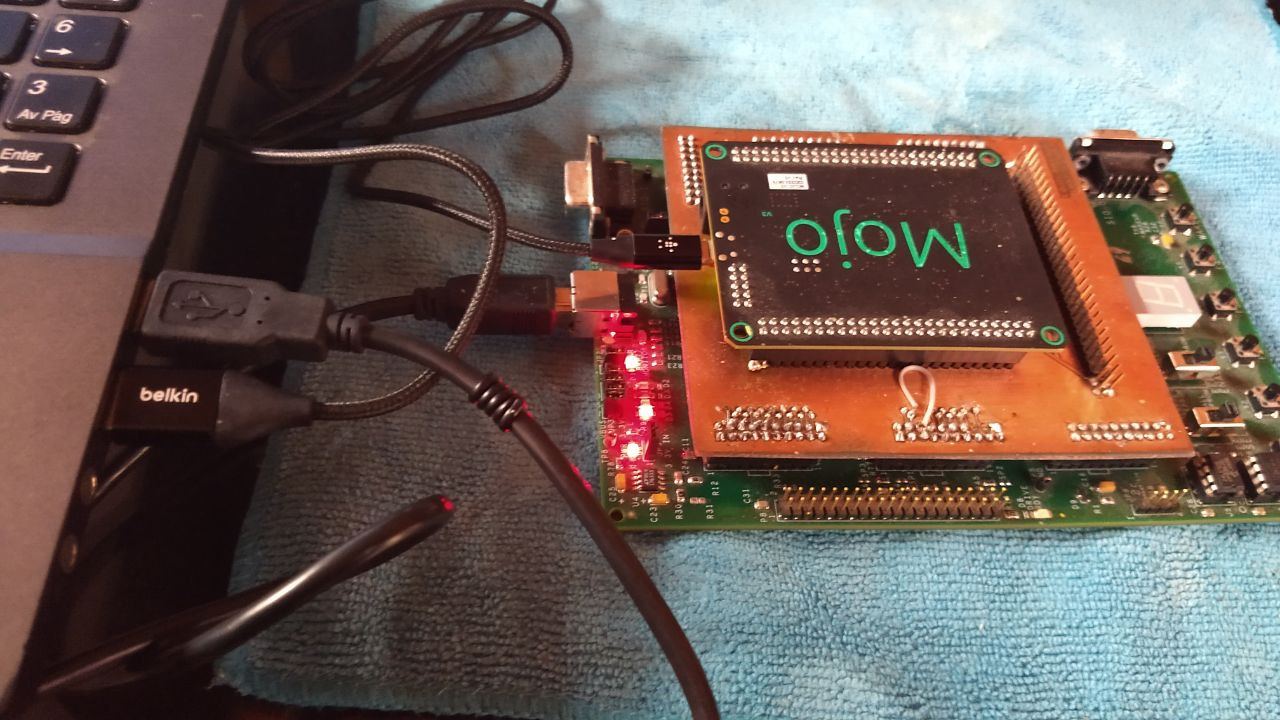
\includegraphics[width=\textwidth]{sistema2}
\end{frame}
